\documentclass{article}
\usepackage[utf8]{inputenc}
\usepackage[T1]{fontenc}

\usepackage{graphicx}
\usepackage{subcaption}

\usepackage{ifxetex}
\ifxetex
  \usepackage{fontspec}
\else
  \usepackage[T1]{fontenc}
  \usepackage[utf8]{inputenc}
  \usepackage{lmodern}
\fi

\title{Evaluación 2}
\author{Roberto Benard Orci}
\date{26/04/2018}

\begin{document}
\maketitle

\section*{Actividad a realizar}
En esta actividad graficamos el atractor de Lorenz, el cual es un sistema caótico, esto significa que pequeños cambios en las condiciones iniciales afectaran de forma significativa el resultado del las ecuaciones. 

El atractor esta compuesto por las siguientes ecuaciones:

 \begin{equation}
 \frac{dx}{dt} =\sigma (y-x)
 \end{equation}
 \begin{equation}
 \frac{dy}{dt} =x (\rho-z)-y
 \end{equation}
  \begin{equation}
 \frac{dz}{dt} =xy-\beta z
 \end{equation}

Donde $\sigma$, $\beta$ y $\rho$ son parámetros que describen diferentes cosas.

\subsection*{Act.1}

En la primera parte utilizamos el código de Geoff Boeing para graficar las visualizaciones y animación del atractor de Lorenz que tiene en los dos casos, estas son la misma gráfica, solo que la animación muestra marco por marco como se llego a la visualización:

\begin{center}
	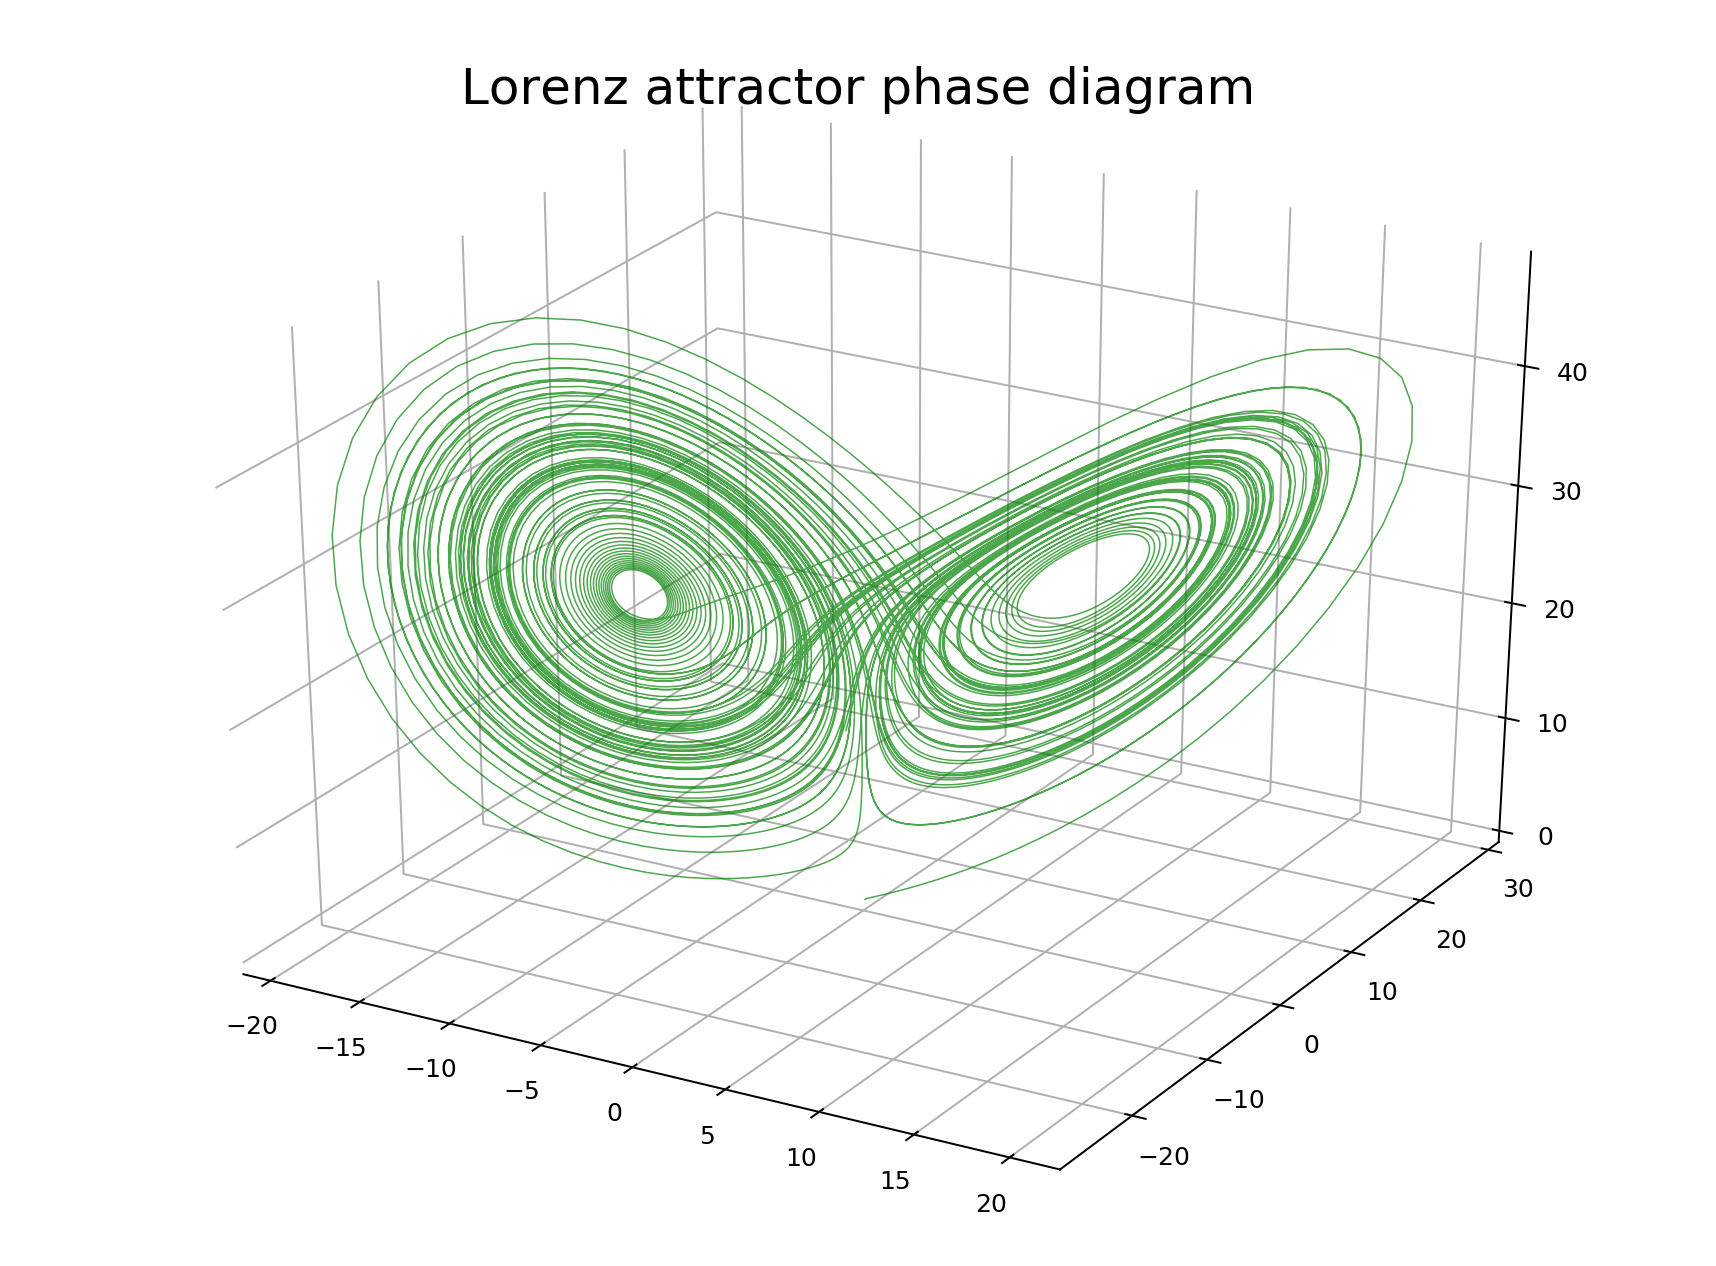
\includegraphics[width=10cm]{lorenz-attractor-3d.png}
    
\end{center}
\vspace{0.3cm}

En esta parte utilizamos los siguientes valores para los parámetros: $\sigma$\textit{=10}, $\beta$\textit{=8/3} , $\rho$\textit{=28}.

Como se puede observar, el atractor muestra dos puntos que son orbitados, en el movimiento cambia la órbita.

\vspace{0.4cm}

También graficamos las siguientes fases. 

\begin{center}
	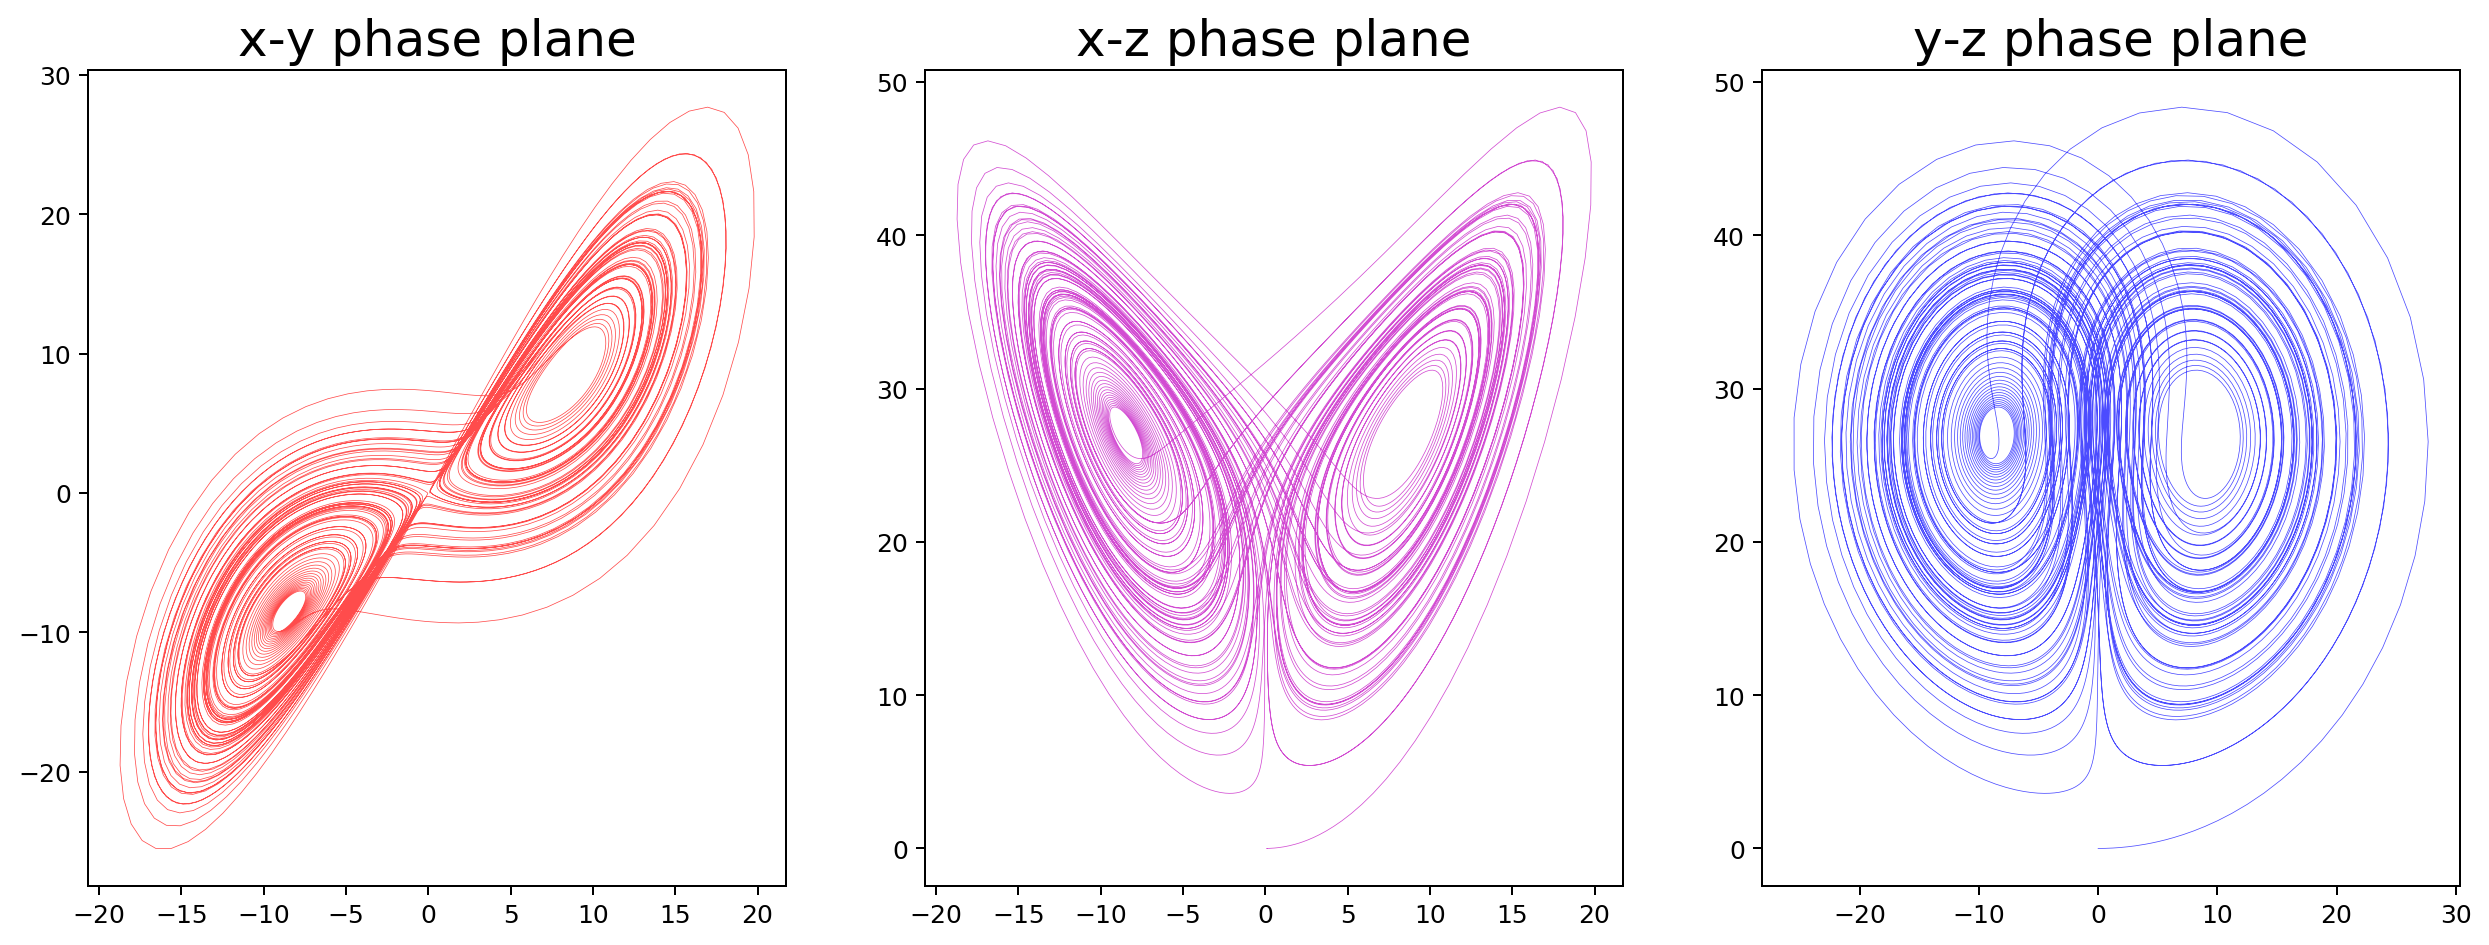
\includegraphics[width=10cm]{lorenz-attractor-phase-plane.png}
    
\end{center}
\vspace{0.3cm}



\subsection*{Act.2}

Aquí construimos las gráficas bidimencionales de las soluciones para ver la evolución temporal de una condición inicial como función del tiempo.

Primero se muestran las 3 gráficas separadas, y luego una gráfica que contiene las tres, un poco mas estirada para apreciar mejor los cambios.


\begin{center}
	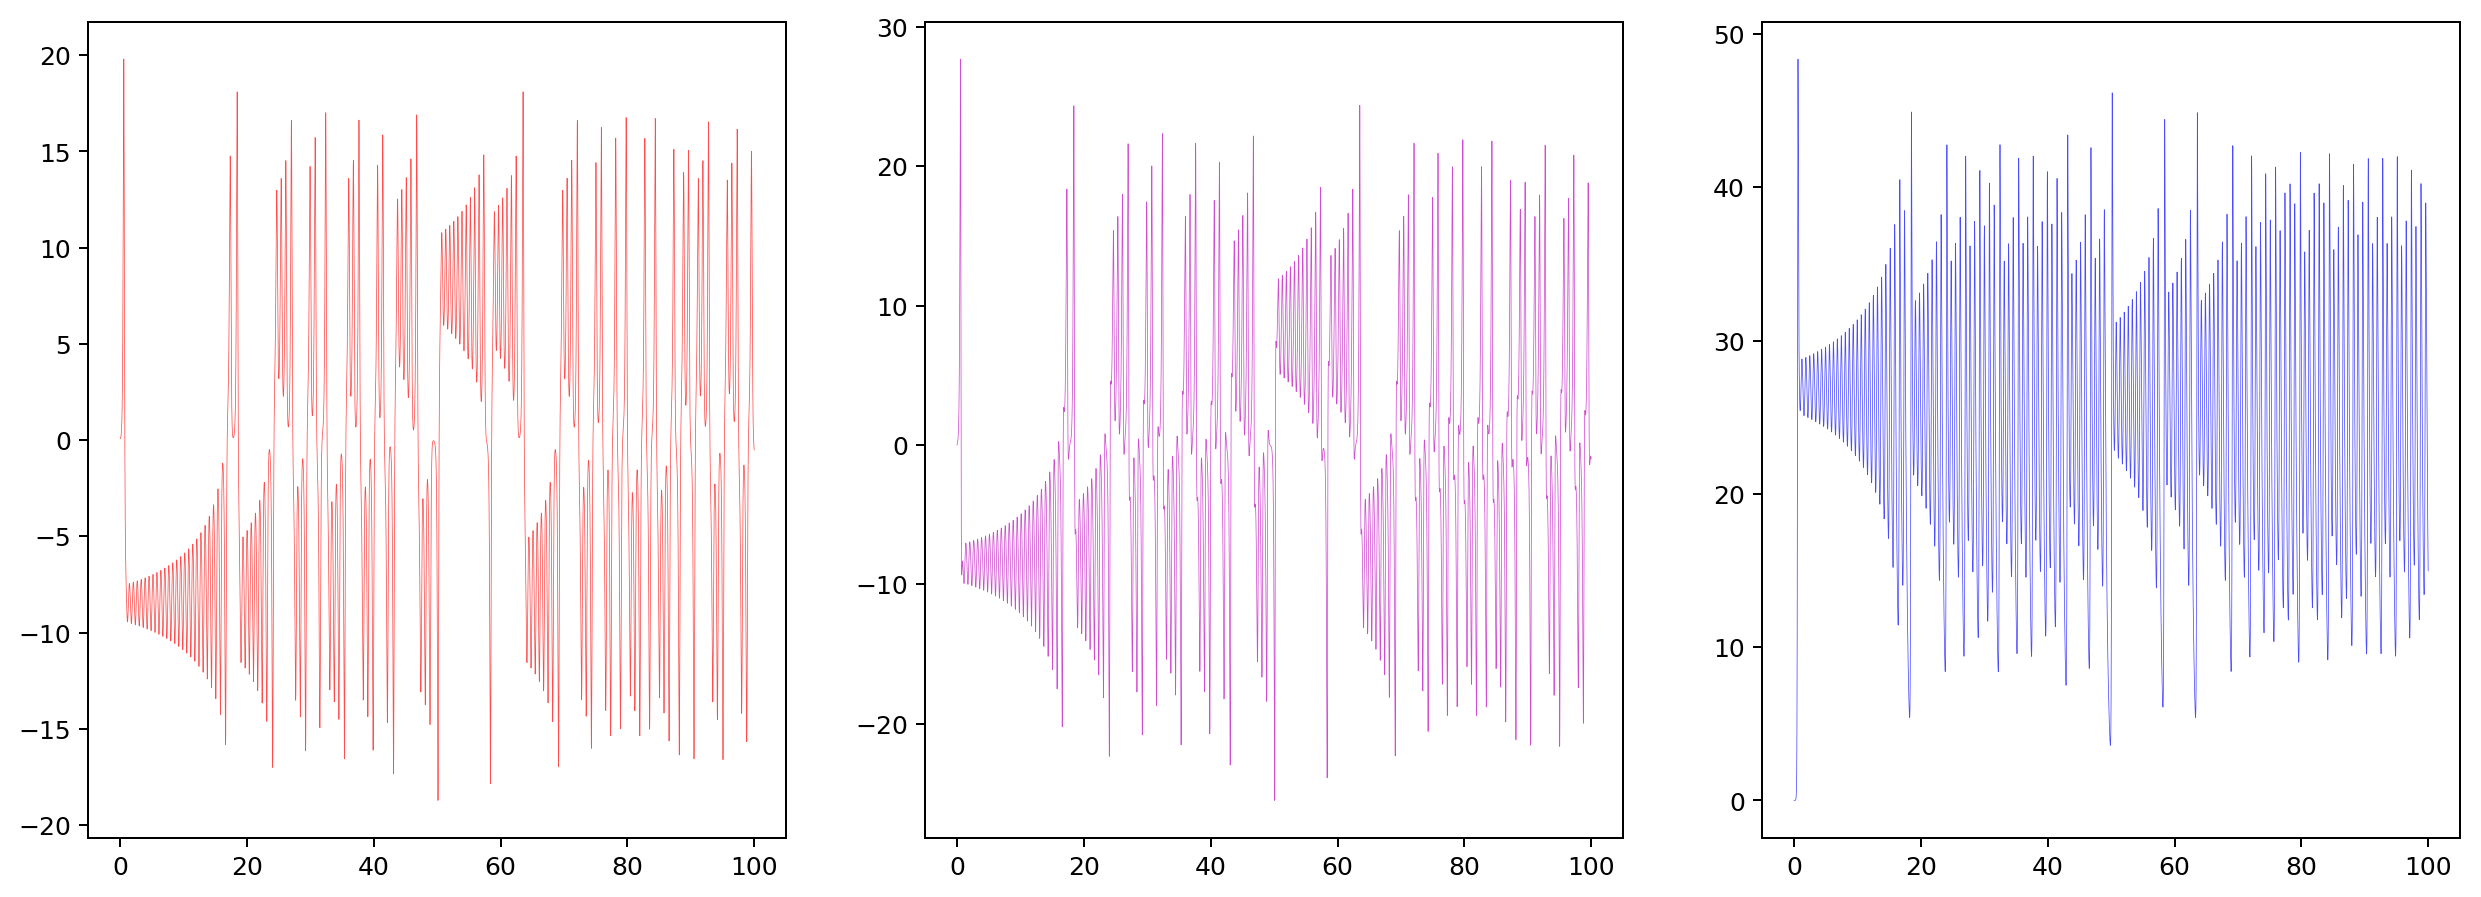
\includegraphics[width=10cm]{ev-temporal.png}
    
\end{center}
\vspace{0.3cm}

\begin{center}
	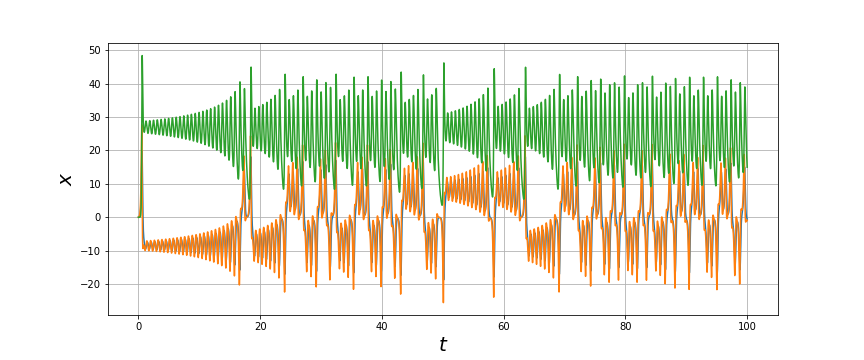
\includegraphics[width=10cm]{ev-temporal-mix.png}
    
\end{center}
\vspace{0.3cm}



\subsection*{Act.3}

Para la actividad 3 hacemos lo mismo que en la 1 y 2, solo que ahora con diferentes parámetros ($\sigma$\textit{=28}, $\beta$\textit{=4} , $\rho$\textit{=46.92}).

Estos fueron los resultados:

\begin{center}
	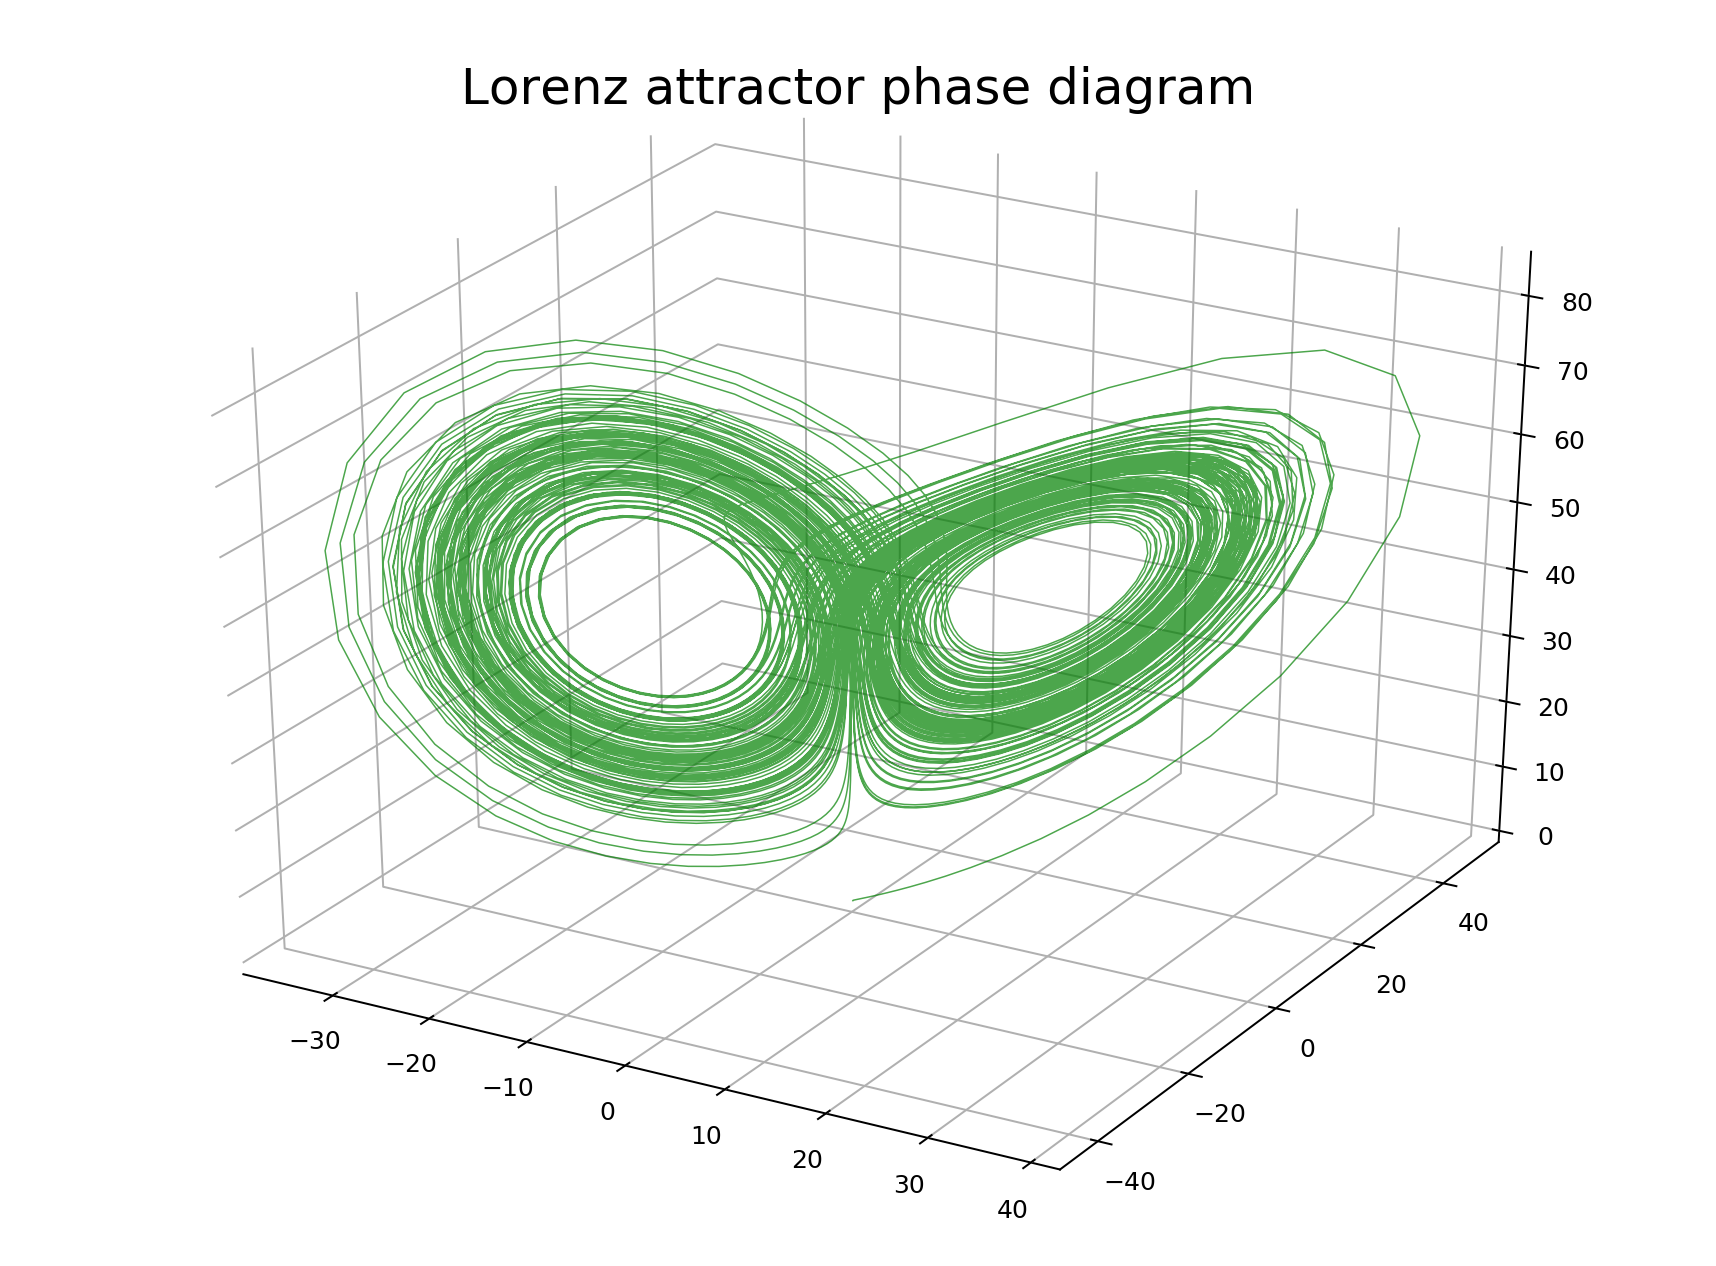
\includegraphics[width=10cm]{lorenz-attractor-3d-2nd.png}
    
\end{center}
\vspace{0.3cm}

\begin{center}
	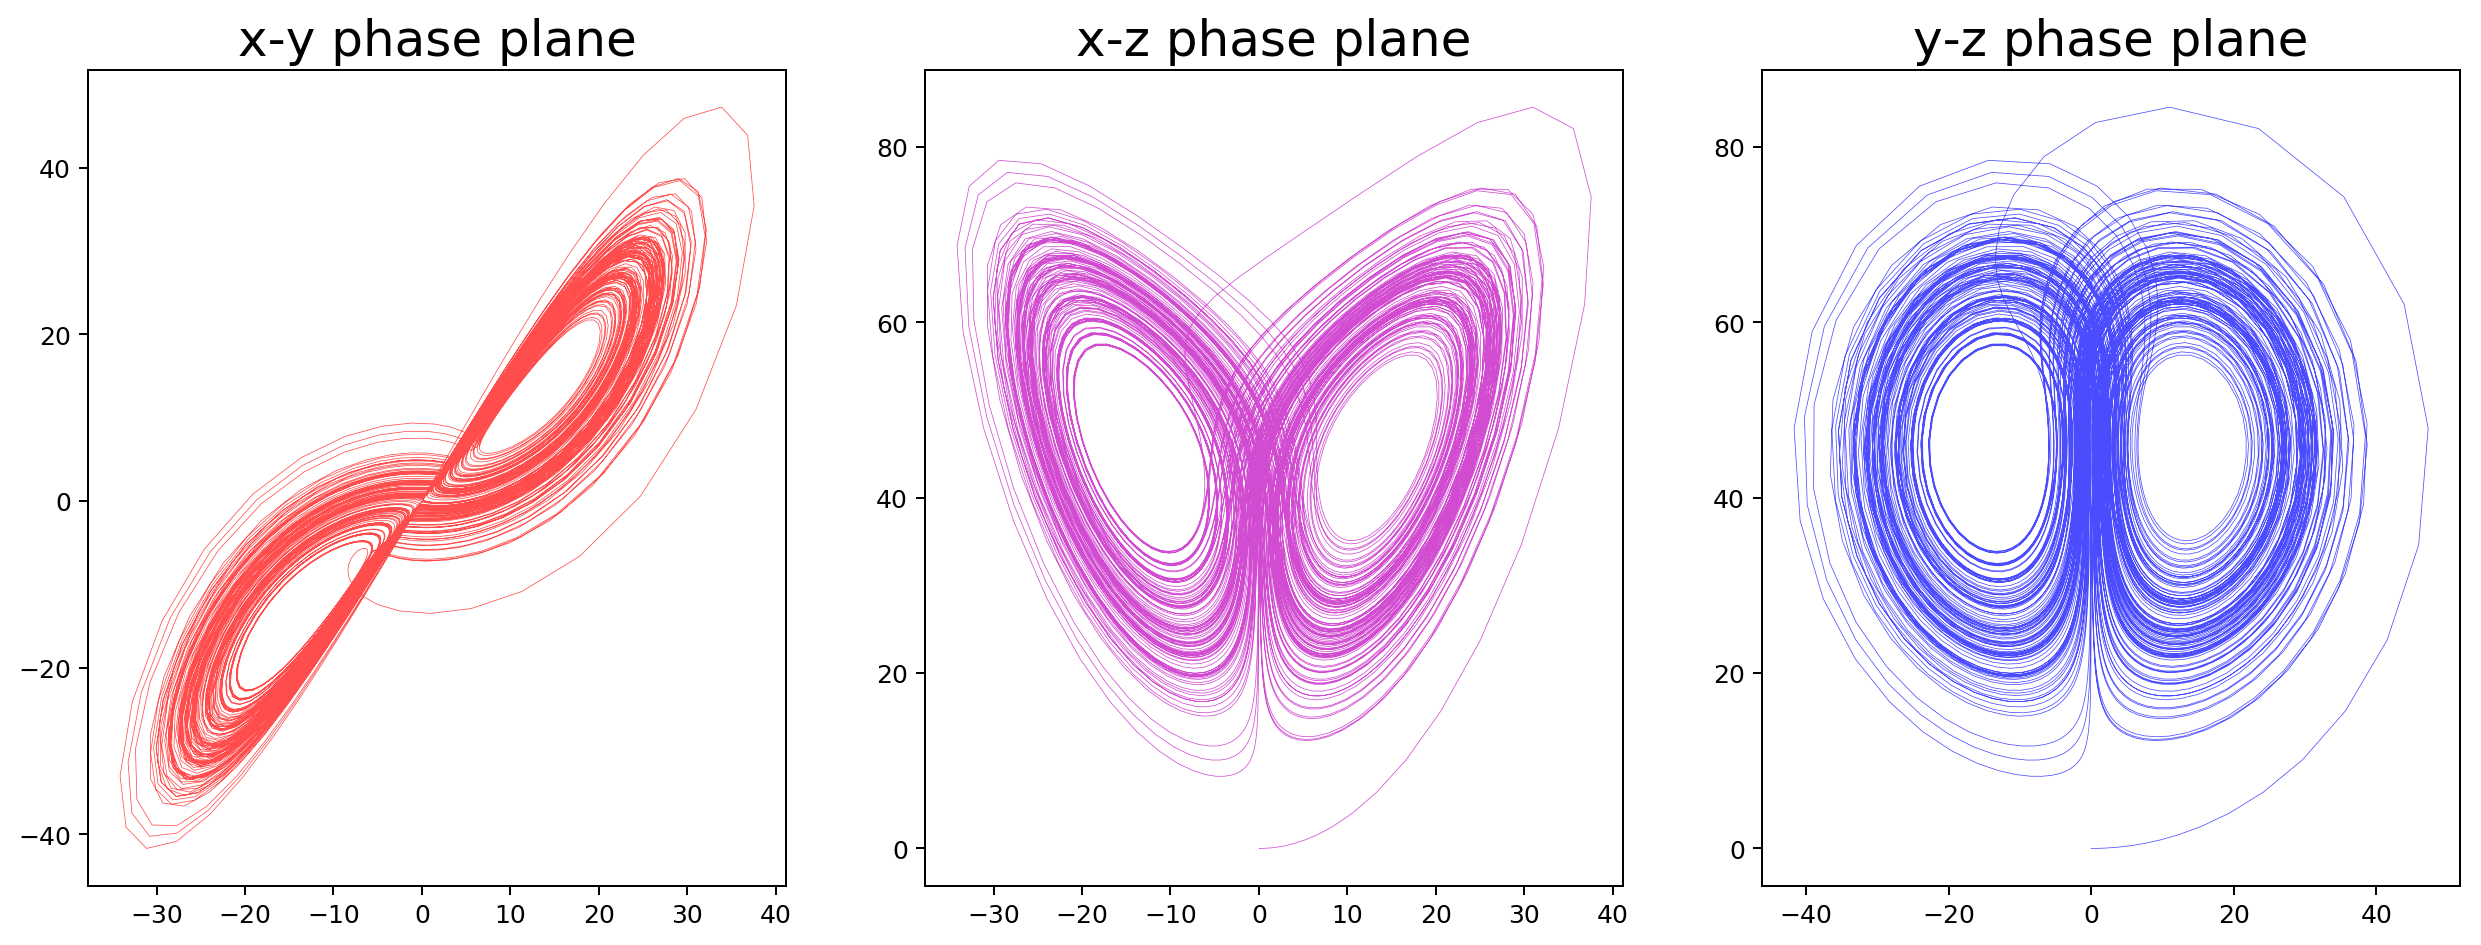
\includegraphics[width=10cm]{lorenz-attractor-phase-plane-2nd.png}
    
\end{center}
\vspace{0.3cm}

\begin{center}
	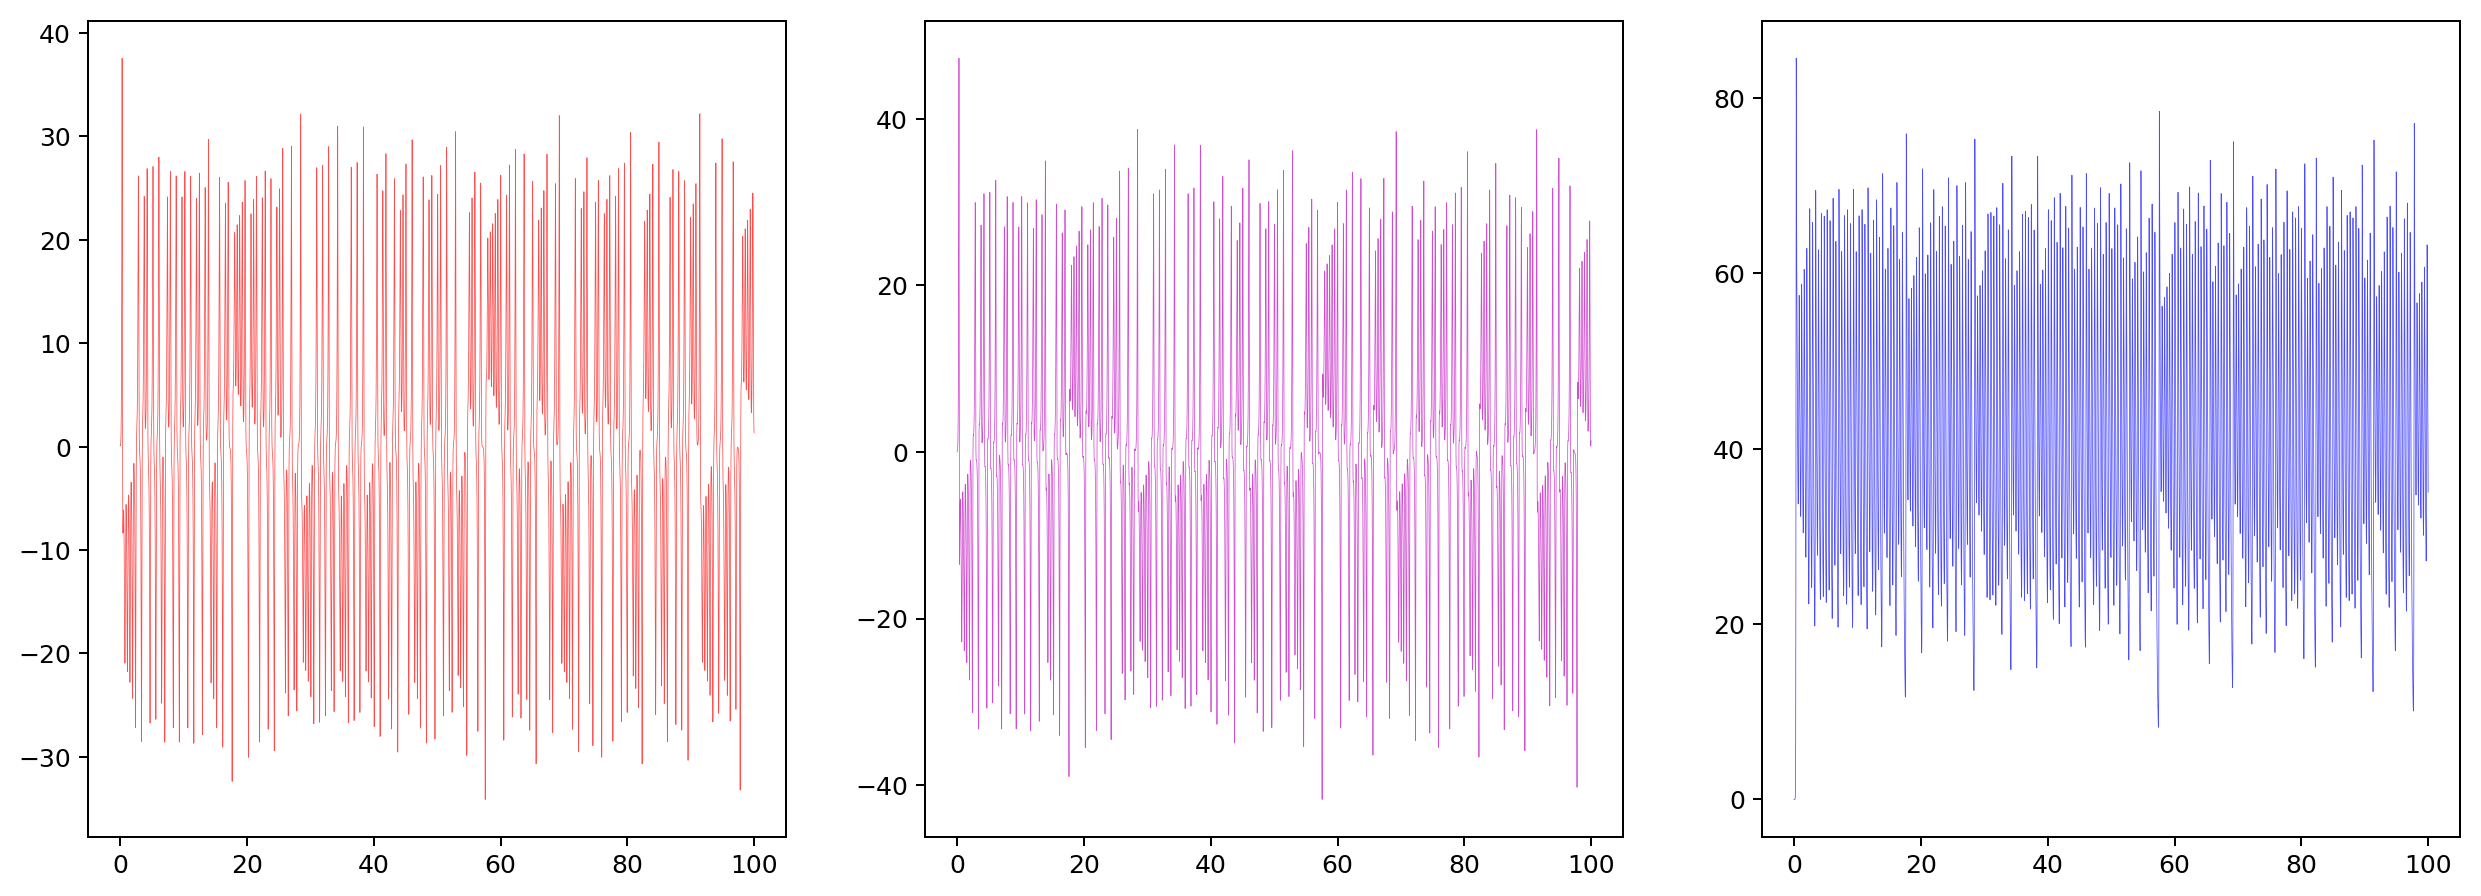
\includegraphics[width=10cm]{ev-temporal-2nd.png}
    
\end{center}
\vspace{0.3cm}

\begin{center}
	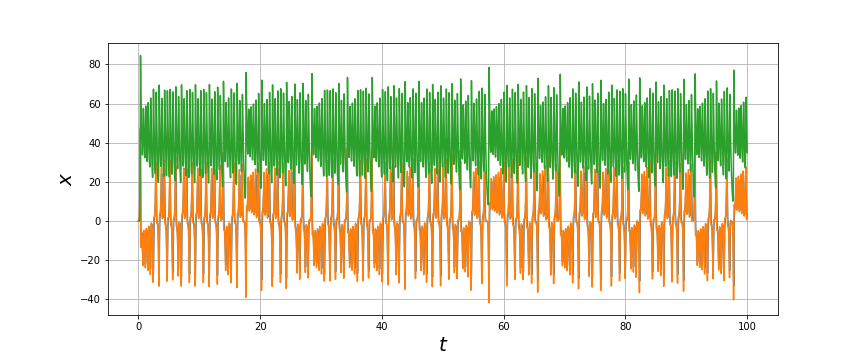
\includegraphics[width=10cm]{ev-temporal-mix-2nd.png}
    
\end{center}
\vspace{0.3cm}

A comparación del anterior, las órbitas son mas grandes y estan ligeramente inclinadas, las fases se ven mas \textit{"densas"}, y las gráficas bidimencionales parecen ser mas caóticas, tiende a cambiar de órbita mas rápido

\subsection*{Act.4}

Por ultimo, en la actividad 4 usamos los parámetros ($\sigma$\textit{=10}, $\beta$\textit{=8/3} , $\rho$\textit{=99.96}).


\begin{center}
	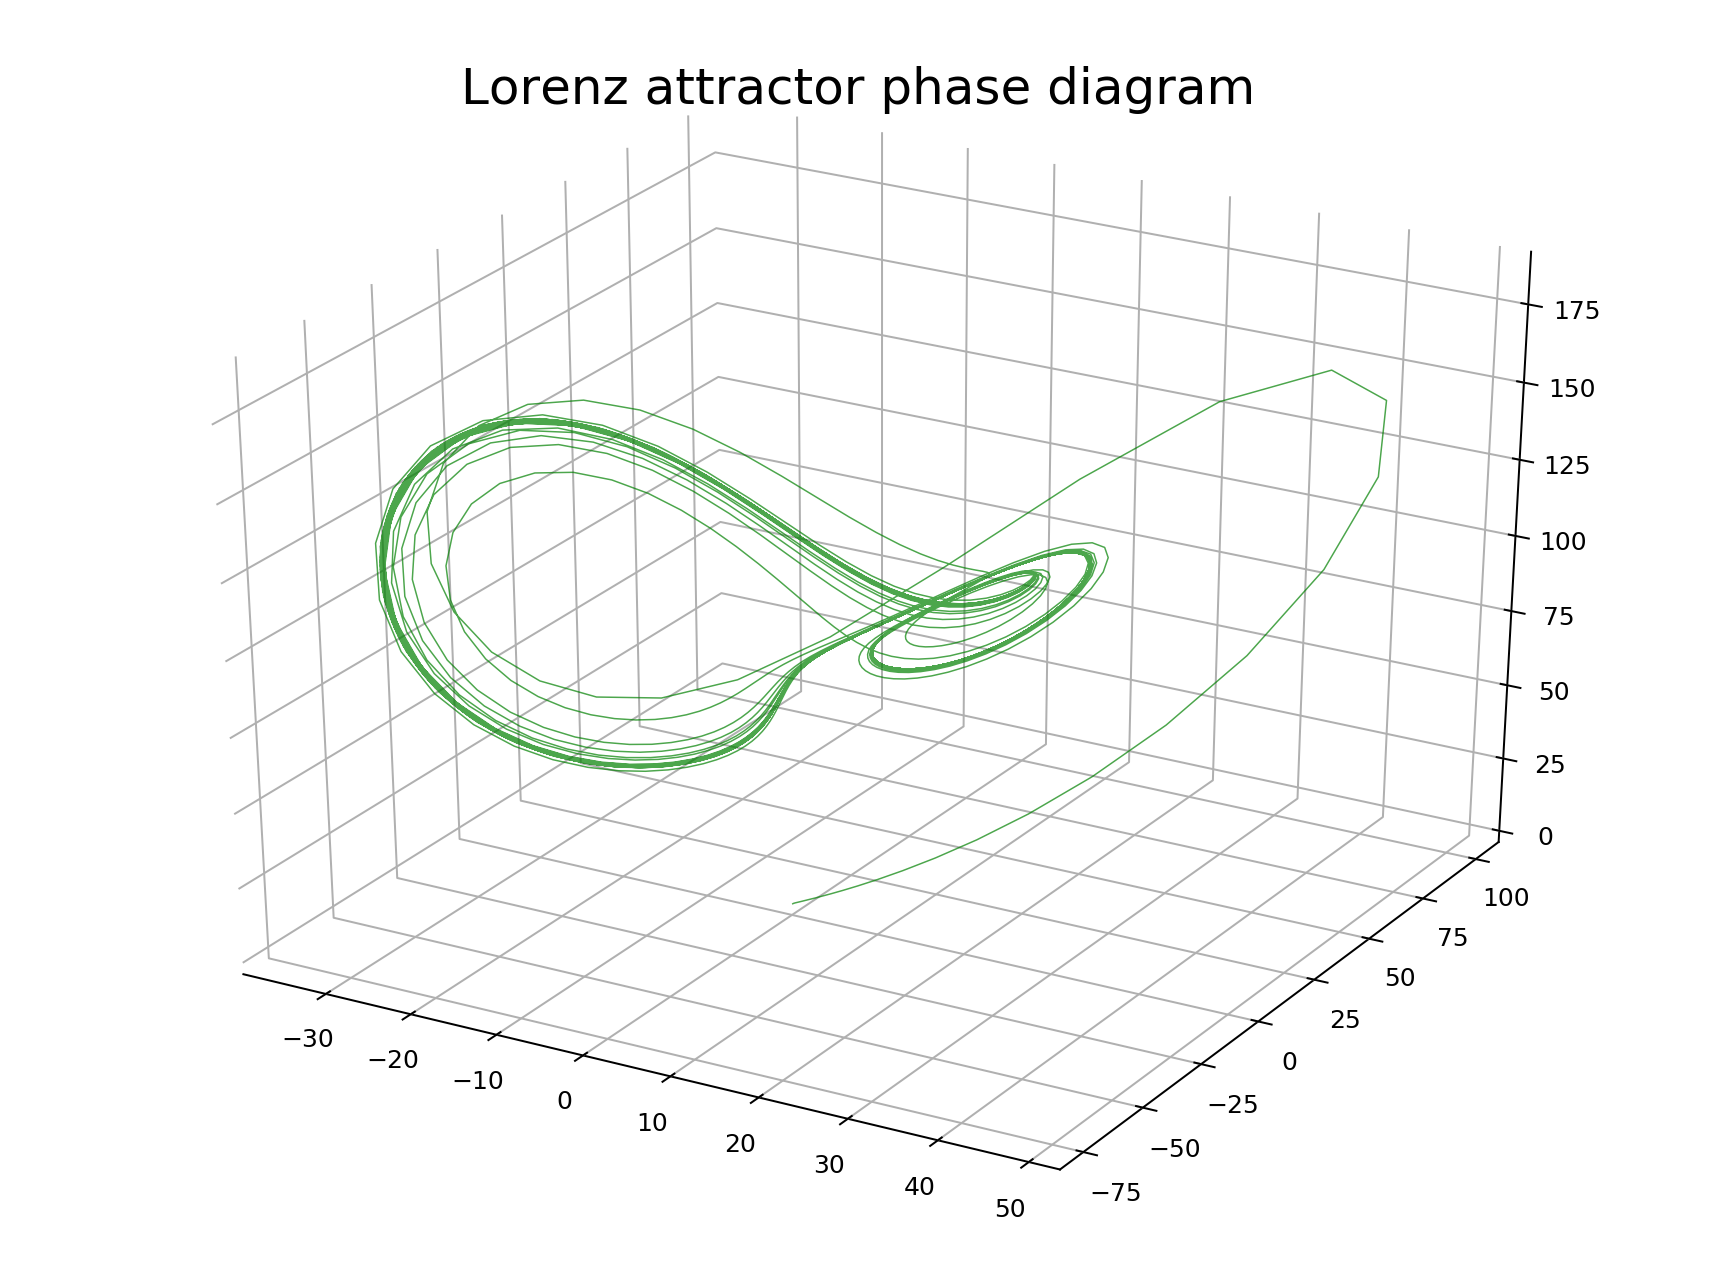
\includegraphics[width=10cm]{lorenz-attractor-3d-3rd.png}
    
\end{center}
\vspace{0.3cm}

\begin{center}
	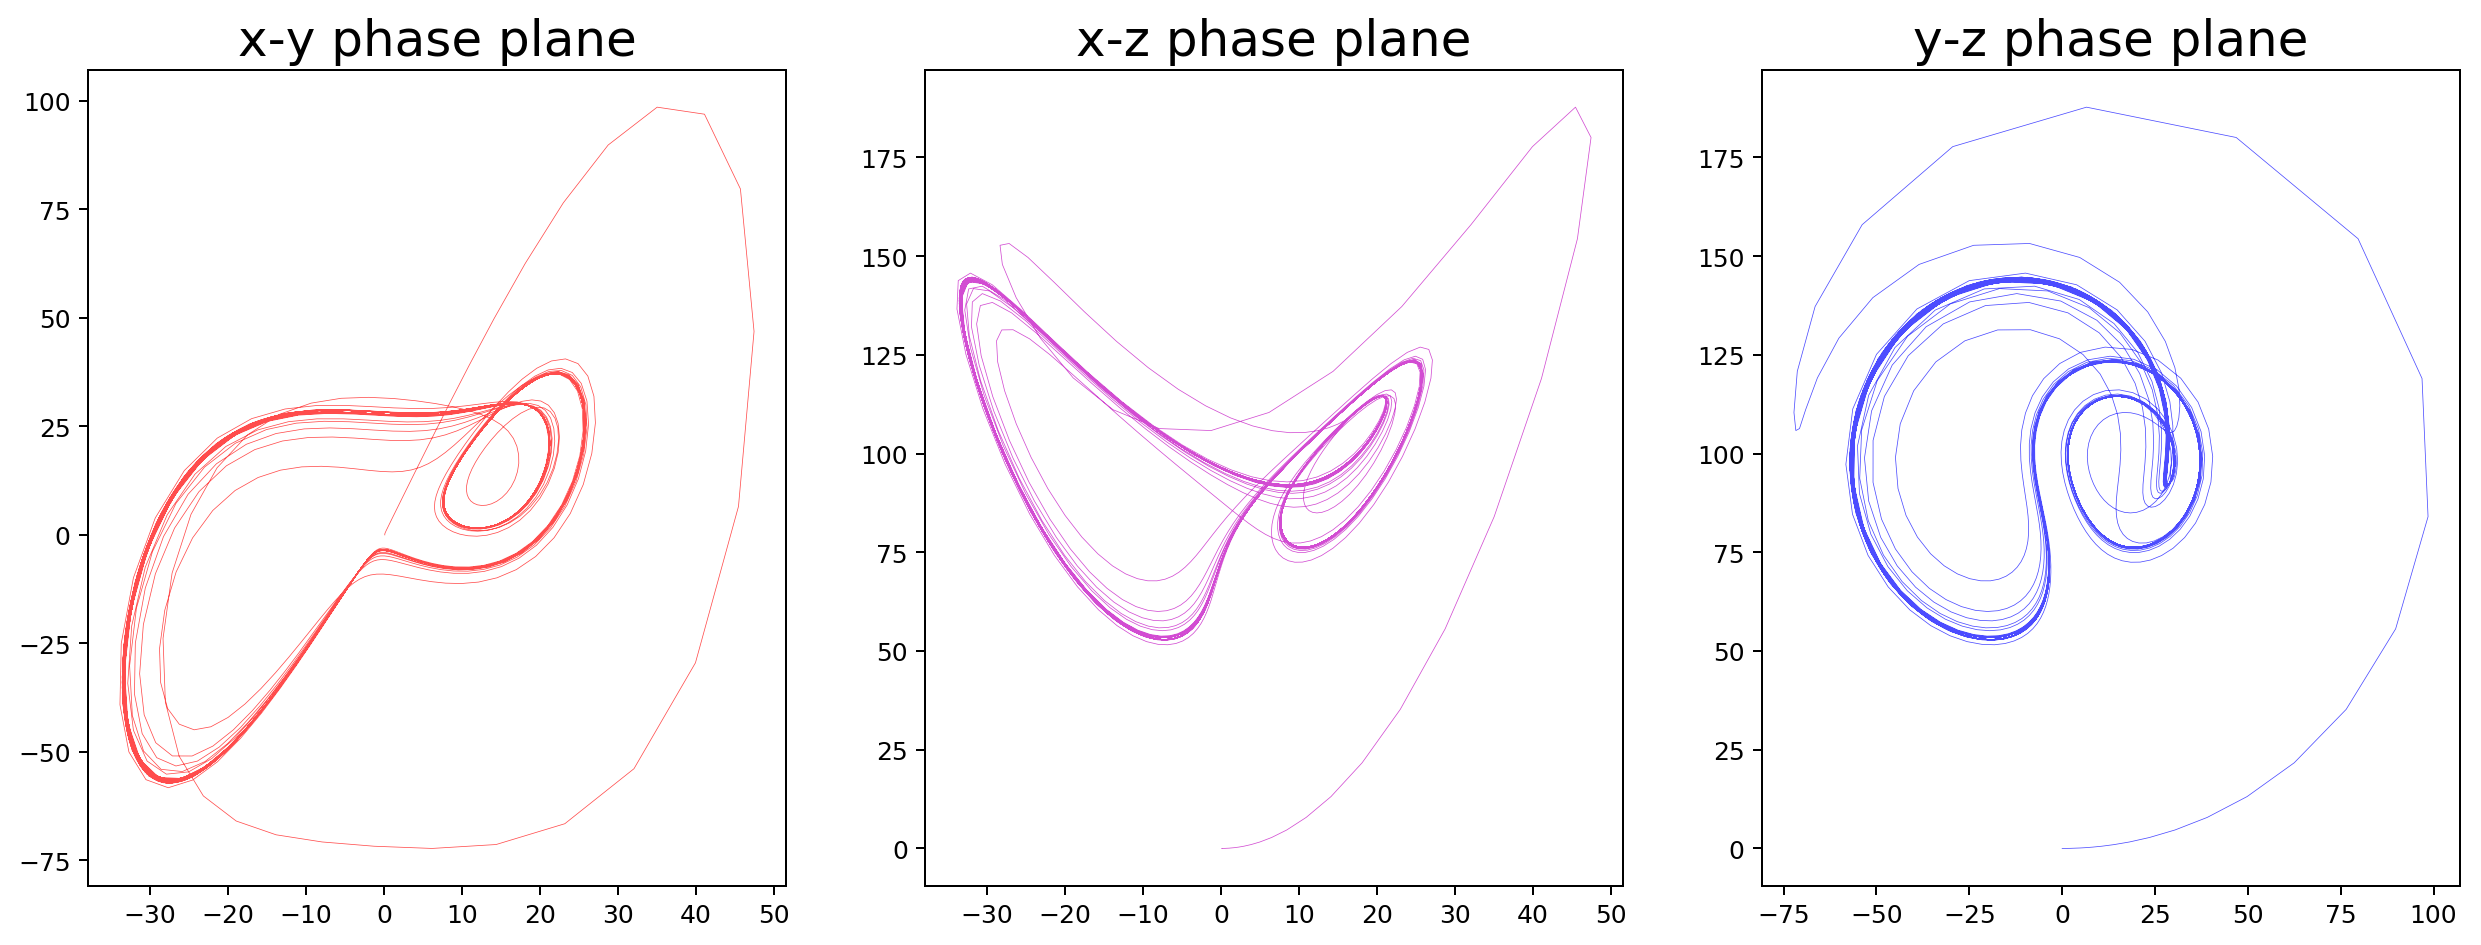
\includegraphics[width=10cm]{lorenz-attractor-phase-plane-3rd.png}
    
\end{center}
\vspace{0.3cm}

\begin{center}
	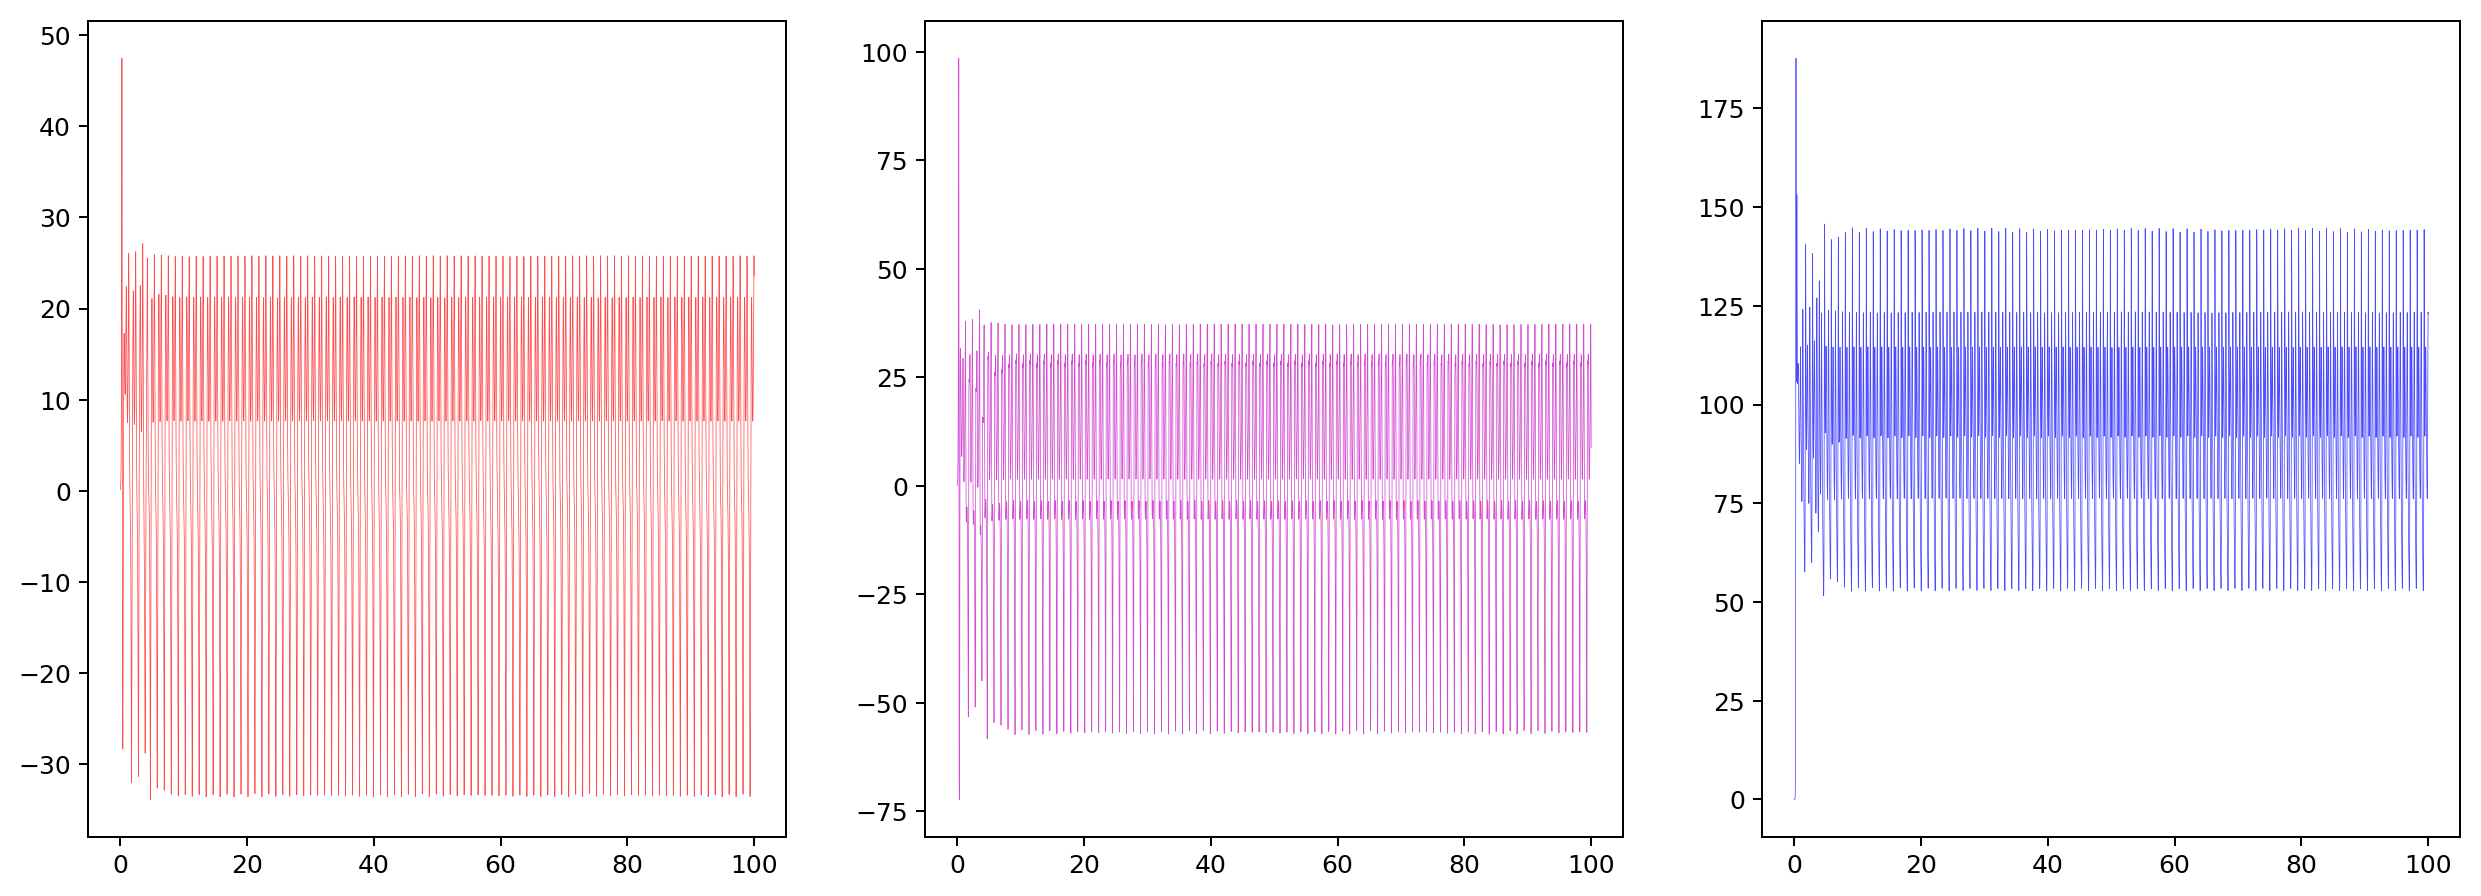
\includegraphics[width=10cm]{ev-temporal-3rd.png}
    
\end{center}
\vspace{0.3cm}

\begin{center}
	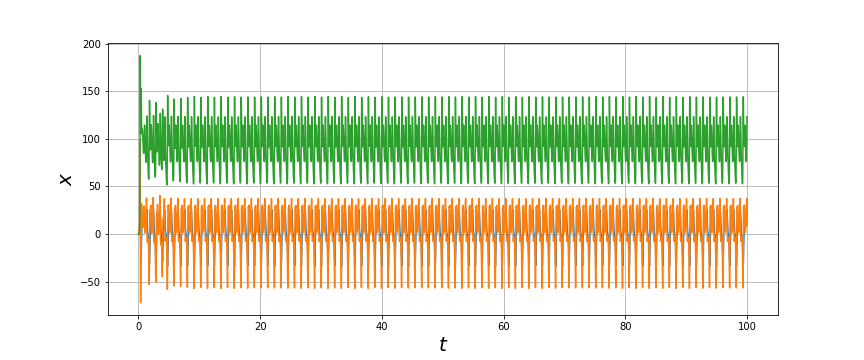
\includegraphics[width=10cm]{ev-temporal-mix-3rd.png}
    
\end{center}
\vspace{0.3cm}

En esta gráfica parece que los atractores actúan de una manera que parece mas \textit{"fuertes"}, me recuerdan a la forma en que simulan el paso de cometas a objetos masivos, pasa muy rápido dando una vuelta cerrada, y luego se tarda mucho en regresar pero con una órbita mas grande. Las graficas de fase apuntan a algo parecido pero solo al verlo de cierto angulo, no en los planos \textit{x}, \textit{y} y \textit{z}.

Las gráficas bidimencionales parecen tener un movimiento periódico, esto también se puede ver al combinar estas gráficas.

\section*{Conclusión}
Para muchos sistemas representados por ecuaciones diferenciales, uno puede encontrar distintos códigos para visualizar estos sistemas y entender mejor como funcionan y que pueden representar.  

\section*{Bibliografía}

\begin{verbatim}
Lorenz system. (2018, April 14). Retrieved from https://en.wikipedia.
org/wiki/Lorenz_system 
\end{verbatim}
%https://en.wikipedia.org/wiki/Lorenz_system

\begin{verbatim}
Gboeing, A. (2017, January 02). Animating the Lorenz Attractor with
Python. Retrieved from http://geoffboeing.com/2016/12/animating-
lorenz-attractor-python/ 
\end{verbatim}
%http://geoffboeing.com/2016/12/animating-lorenz-attractor-python/

\begin{verbatim}
G. (n.d.). Gboeing/lorenz-system. Retrieved from https://github.com/
gboeing/lorenz-system 
\end{verbatim}
%https://github.com/gboeing/lorenz-system

\end{document}